% !TeX root = RJwrapper.tex
\title{Exploring Alternatives to WGCNA in Neuroscience}
\author{by Benjamin Koppe}

\maketitle

\abstract{
Weighted Gene Co-expression Network Analysis (WGCNA) is a well-established cornerstone for understanding gene expression patterns and uncovering the systems-level functionality of genes. However, WGCNA has a number of limitations, making application often tedious and difficult. This drives the need for more efficient alternatives. This paper details an investigation into the efficacy of some of these alternatives, focusing particularily CEMiTool: a novel approach in gene co-expression analysis. Files for this project can be found in its \href{https://github.com/benkoppe/wgcna-alternatives/}{GitHub Repository}.
}


\section{Introduction}

\subsection{WGCNA}
\label{subsec: WGCNA}
The process of clustering genes into modules is an important tool to understand complex biological systems. Gene clustering allows researchers to unravel complex interactions between genes and understand their impact. In neuroscience, for example, it is commonly used to analyze brain development, disorders, and behavior. WGCNA is an R package developed to perform this complex process by constructing networks (graphs) of genes based on the similarity of their expression patterns.~\cite{wgcna} WGCNA is by far the most popular and widely used package in its class.

However, WGCNA poses a multitude of problems.~\cite{cem} WGCNA has a long and tedious workflow that is time-consuming to configure and generalize, often requiring large amounts of code. This requires users to spend time constantly surveying for problems and errors. WGCNA also forces users to manually select a number of different parameters and filter input genes by hand. This process impacts reproducibility, as parameter selection is highly influential in output, and places the burden on researchers to justify the selection of each parameter. It also makes the already difficult workflow much harder to automate. Finally, WGCNA is limited in options for functional analyses.

In summary, WGCNA is weighed down by its high barriers to entry, which can be problematic for bioinformatics researchers both with and without technical and computing knowledge. To alleviate these problems, this investigation was launched to evaluate the number of alternative packages that have been written since the introduction of WGCNA.

\subsection{CEMiTool}
The Bioconductor package CEMiTool \cite{cem} was selected as the primary alternative in this investigation. CEMiTool was created primarily to address problems with WGCNA. The problems listed in \ref{subsec: WGCNA} are all referenced in CEMiTool's introductory paper and used as a motivation for the package's development.

\begin{quote}
    ``[CEMiTool] allows users to easily identify and analyze co-expression modules in a fully automated manner [and] [...] provides users with a novel unsupervised gene filtering method, automated parameter selection for identifying modules, enrichment and module functional analyses, as well as integration with interactome data. [It] then reports everything in HTML web pages with high-quality plots and interactive tables.'' \cite{cem}
\end{quote}

\noindent CEMiTool's many features and highly simplified and automated workflow make it a very compelling alternative for WGCNA. As such, all implementations and testing shown in this paper will use CEMiTool.


\section{Methods}

\subsection{General Investigation}
Before focusing specifically on CEMiTool, a few packages were assessed in order to create a general overview. Besides CEMiTool, other alternative candidates were BioNERO \cite{bionero}, petal \cite{petal}, and minet \cite{minet}. Later, GWENA \cite{gwena} was also briefly examined. Packages were evaluated primarily from their descriptions in their corresponding papers. Desired properties were ease of use, explicit pathways for comparison to WGCNA results, and explicit implementation details designed to address the primary WGCNA problems listed in \ref{subsec: WGCNA}.

Once CEMiTool was selected, implementation was focused around the development of an optimal simple workflow for dataset analysis. To do this, a 2012 microarray dataset \cite{dataset} was used for all testing. A slightly reformatted copy of the dataset is available in the project repository.

\subsection{R}
\label{subsec: R}
Due to its strength in statistical analysis, large community, and close association to the Bioconductor project, among other factors, R is the near-universally used language in this area. All co-expression analysis packages examined in this report are written in R. As a result, R is a critical component of this report's methodology, as all implementations must use or interface with R.

An especially notable advantage of R is its high degree of flexibility. R has excellent capabilities for integration with other languages and tools, such as Python, C++, and Java. This is valuable to this study, as it allows for the testing of other languages for a further optimized workflow. Though R has many advantages, its age and design can lead to numerous problems: it is riddled with dangerous inconsistency where many parts disagree; it lacks clear convention and documentation in many cases; its package management completely lacks proper support for dependencies, version control, and environment management; and it suffers from very poor scalability through largely unaddressed problems like name collisions. Problems like these have been well documented and continue to persist over time.~\cite{r_inferno}\cite{r_problems} R's ease of interface, however, allows us to experiment with solutions that avoid these problems.

\subsection{Python}
\label{subsec: python-intro}
Python was used as a potential alternative to R code in the workflows investigated in this report. As a result, most code in this report is written in Python. Implementing between R and Python is simple and seamless, and Python includes a number of advantages over R, such as simple and reliable package management, a much higher degree of consistency, and a broader range of libraries such as \texttt{cupy} (for GPU-accelerated computation) and \texttt{PySpark} (for large-scale data processing) that benefit scalability significantly. Though statistical analysis is not as closely tied with the language's design philosophy as with R, this project's code was implemented in Python with the hope that it can benefit greatly from the language's generality and highly-enforced standards, leading to a better overall workflow.

\subsection{Visual Studio Code (VSCode)}
VSCode was used as the Integrated Development Environment (IDE) throughout this process. This means that all code was written and run in the VSCode environment. VSCode's extremely large community and lightweight implementation makes it the only IDE with comprehensive support of nearly any language or file type that can be encountered. This was especially useful for this project, as it allowed for R, Python, and Jupyter Notebook files to be simultaneously edited and run in a single place. VSCode's high modularity and large array of extensions also put it ahead of other IDEs. Some especially useful extensions are Remote-ssh, GitHub Copilot, Prettier, autoDocstring, and Todo Tree.

\subsection{Jupyter Notebooks}
Another benefit of Python is support for Jupyter Notebooks, which allow for inline display of markdown text, runnable code, and dynamic displayed data/analysis. Jupyter Notebooks have built-in caching, where CPU-bound tasks can be isolated to a single block of code, run a single time, and kept cached for use in all other blocks without repeating the calculation. Jupyter Notebooks are also compatible with VSCode. In this project, these notebooks allow for easy and simplistic code demoing and display, and are hosted on Google Colab. All Jupyter Notebooks in this project are also kept in the main repository.


\section{Results}

\subsection{Running CEMiTool}
CEMiTool automates the entire module discovery process with a single function call -- the \texttt{cemitool} function. With this function, a \texttt{cem} object is created, and all future processing is centered around this object. In R, this functionality looks like this:

\begin{example}
  df <- read.delim2("data/probe_data_copy.txt")
  cem <- cemitool(df)
  
  generate_report(cem)
  modules(cem)
  ...
\end{example}

\noindent The only required argument is a gene expression file that contains genes as rows and samples as columns (\texttt{df} in this case). From there, genes are selected from an unsupervised filtering method based on the inverse gamma distribution, a soft-thresholding power $\beta$ is chosen and used to determine a similarity criterion, and the genes are separated into modules using the Dynamic Tree Cut package.~\cite{cem}

The \texttt{cemitool} function accepts a number of additional parameters: filtering and verbose output can be individually enabled or disabled; gene interactions can be provided in an additional file to return network graphs of interacting genes; a sample annotation file can be provided to perform gene set enrichment analysis (GSEA), allowing users to visualize induced or repressed modules in different phenotypes; and a file containing gene sets can be provided to allow for over-representation analysis (ORA) to determine more significant module functions. A number of other parameters are also provided for additional control, but all are optional to provide minimal user responsibility. For reference and ease of comparison, CEMiTool's original paper kept all parameters at their default value. In this analysis, CEMiTool was run with default parameters and no optional files.

\subsection{Visualizing CEMiTool}
\label{subsec: visualizing}
From there, CEMiTool contains multiple built-in plotting and analysis functions. Most notable are its \texttt{diagnostic\_report} and \texttt{generate\_report} functions. Rather than generate simple plots for viewing, these functions generate interactive HTML files that display multiple useful diagnostic plots at once, module data, and full \texttt{cemitool} object parameterization. These files can be viewed in a browser (or in VSCode with the \emph{live\ preview} extension), and because multiple runs don't modify file path, the paths for these HTML files can be left open in the user's browser and conveniently reloaded on each new run of a dataset. An example of these reports can be seen in Figure~\ref{fig:cemi-htmls}.

\begin{figure}[!htb]

  \begin{subfigure}{0.5\textwidth}
    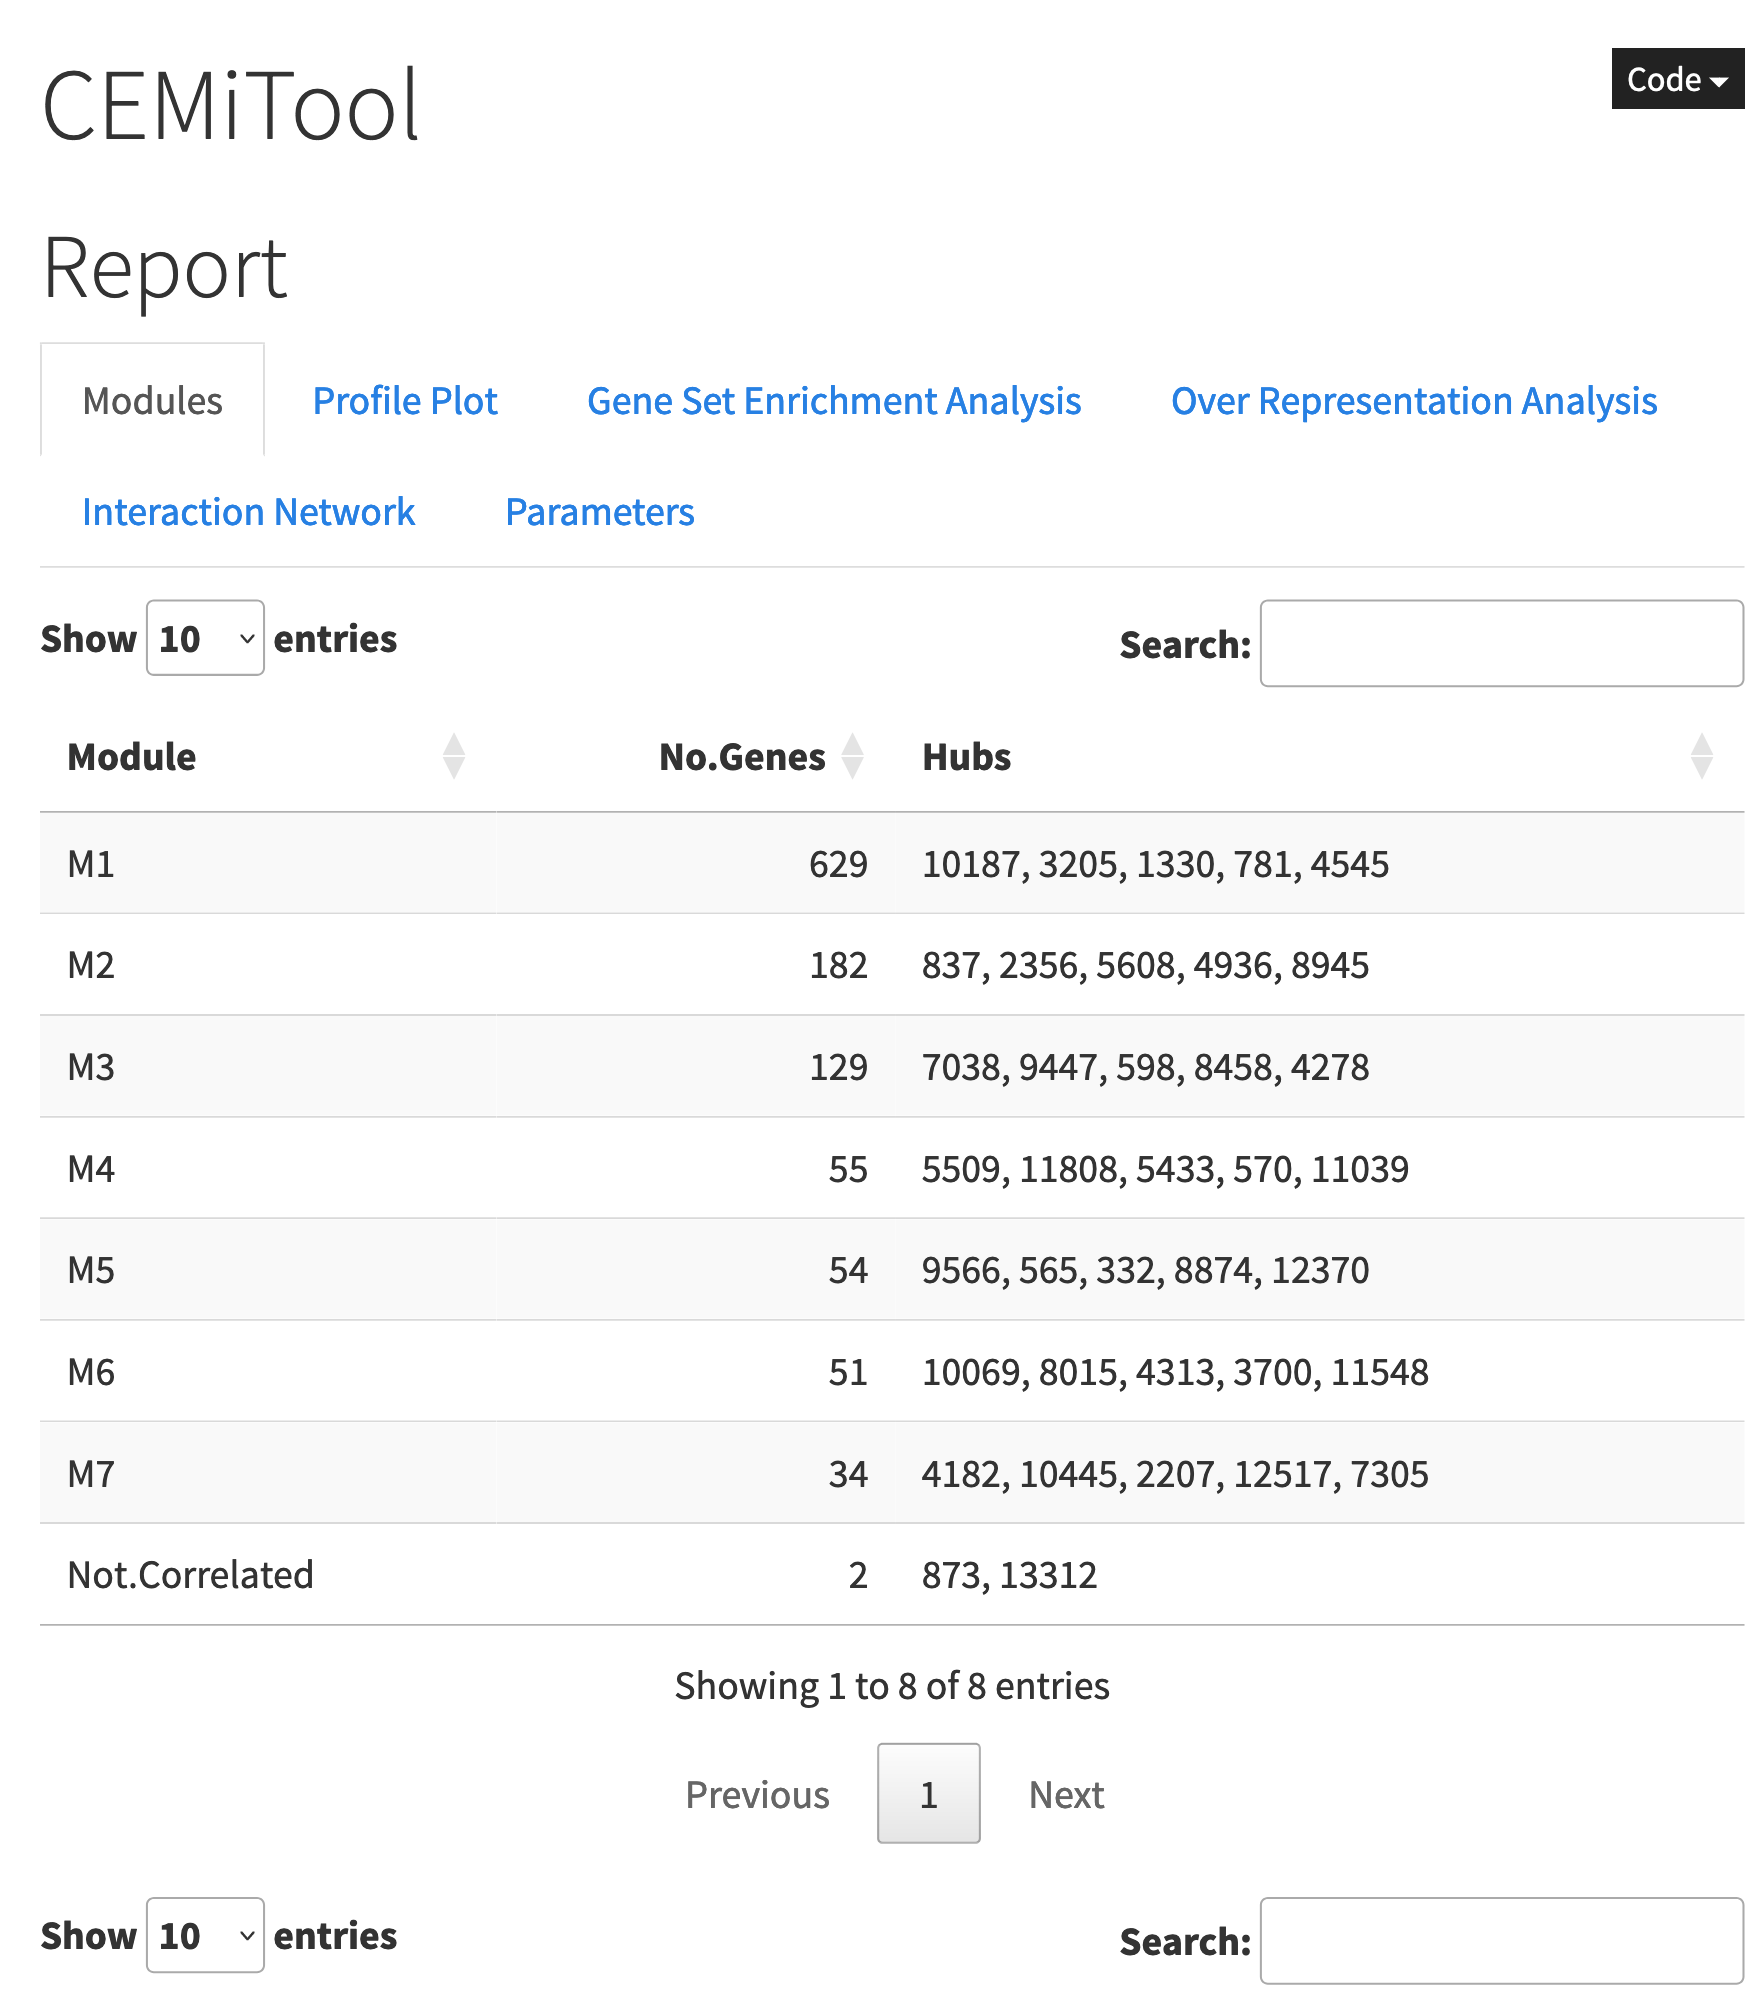
\includegraphics[width=0.9\linewidth]{images/cemi-report} 
  \end{subfigure}
  \begin{subfigure}{0.5\textwidth}
    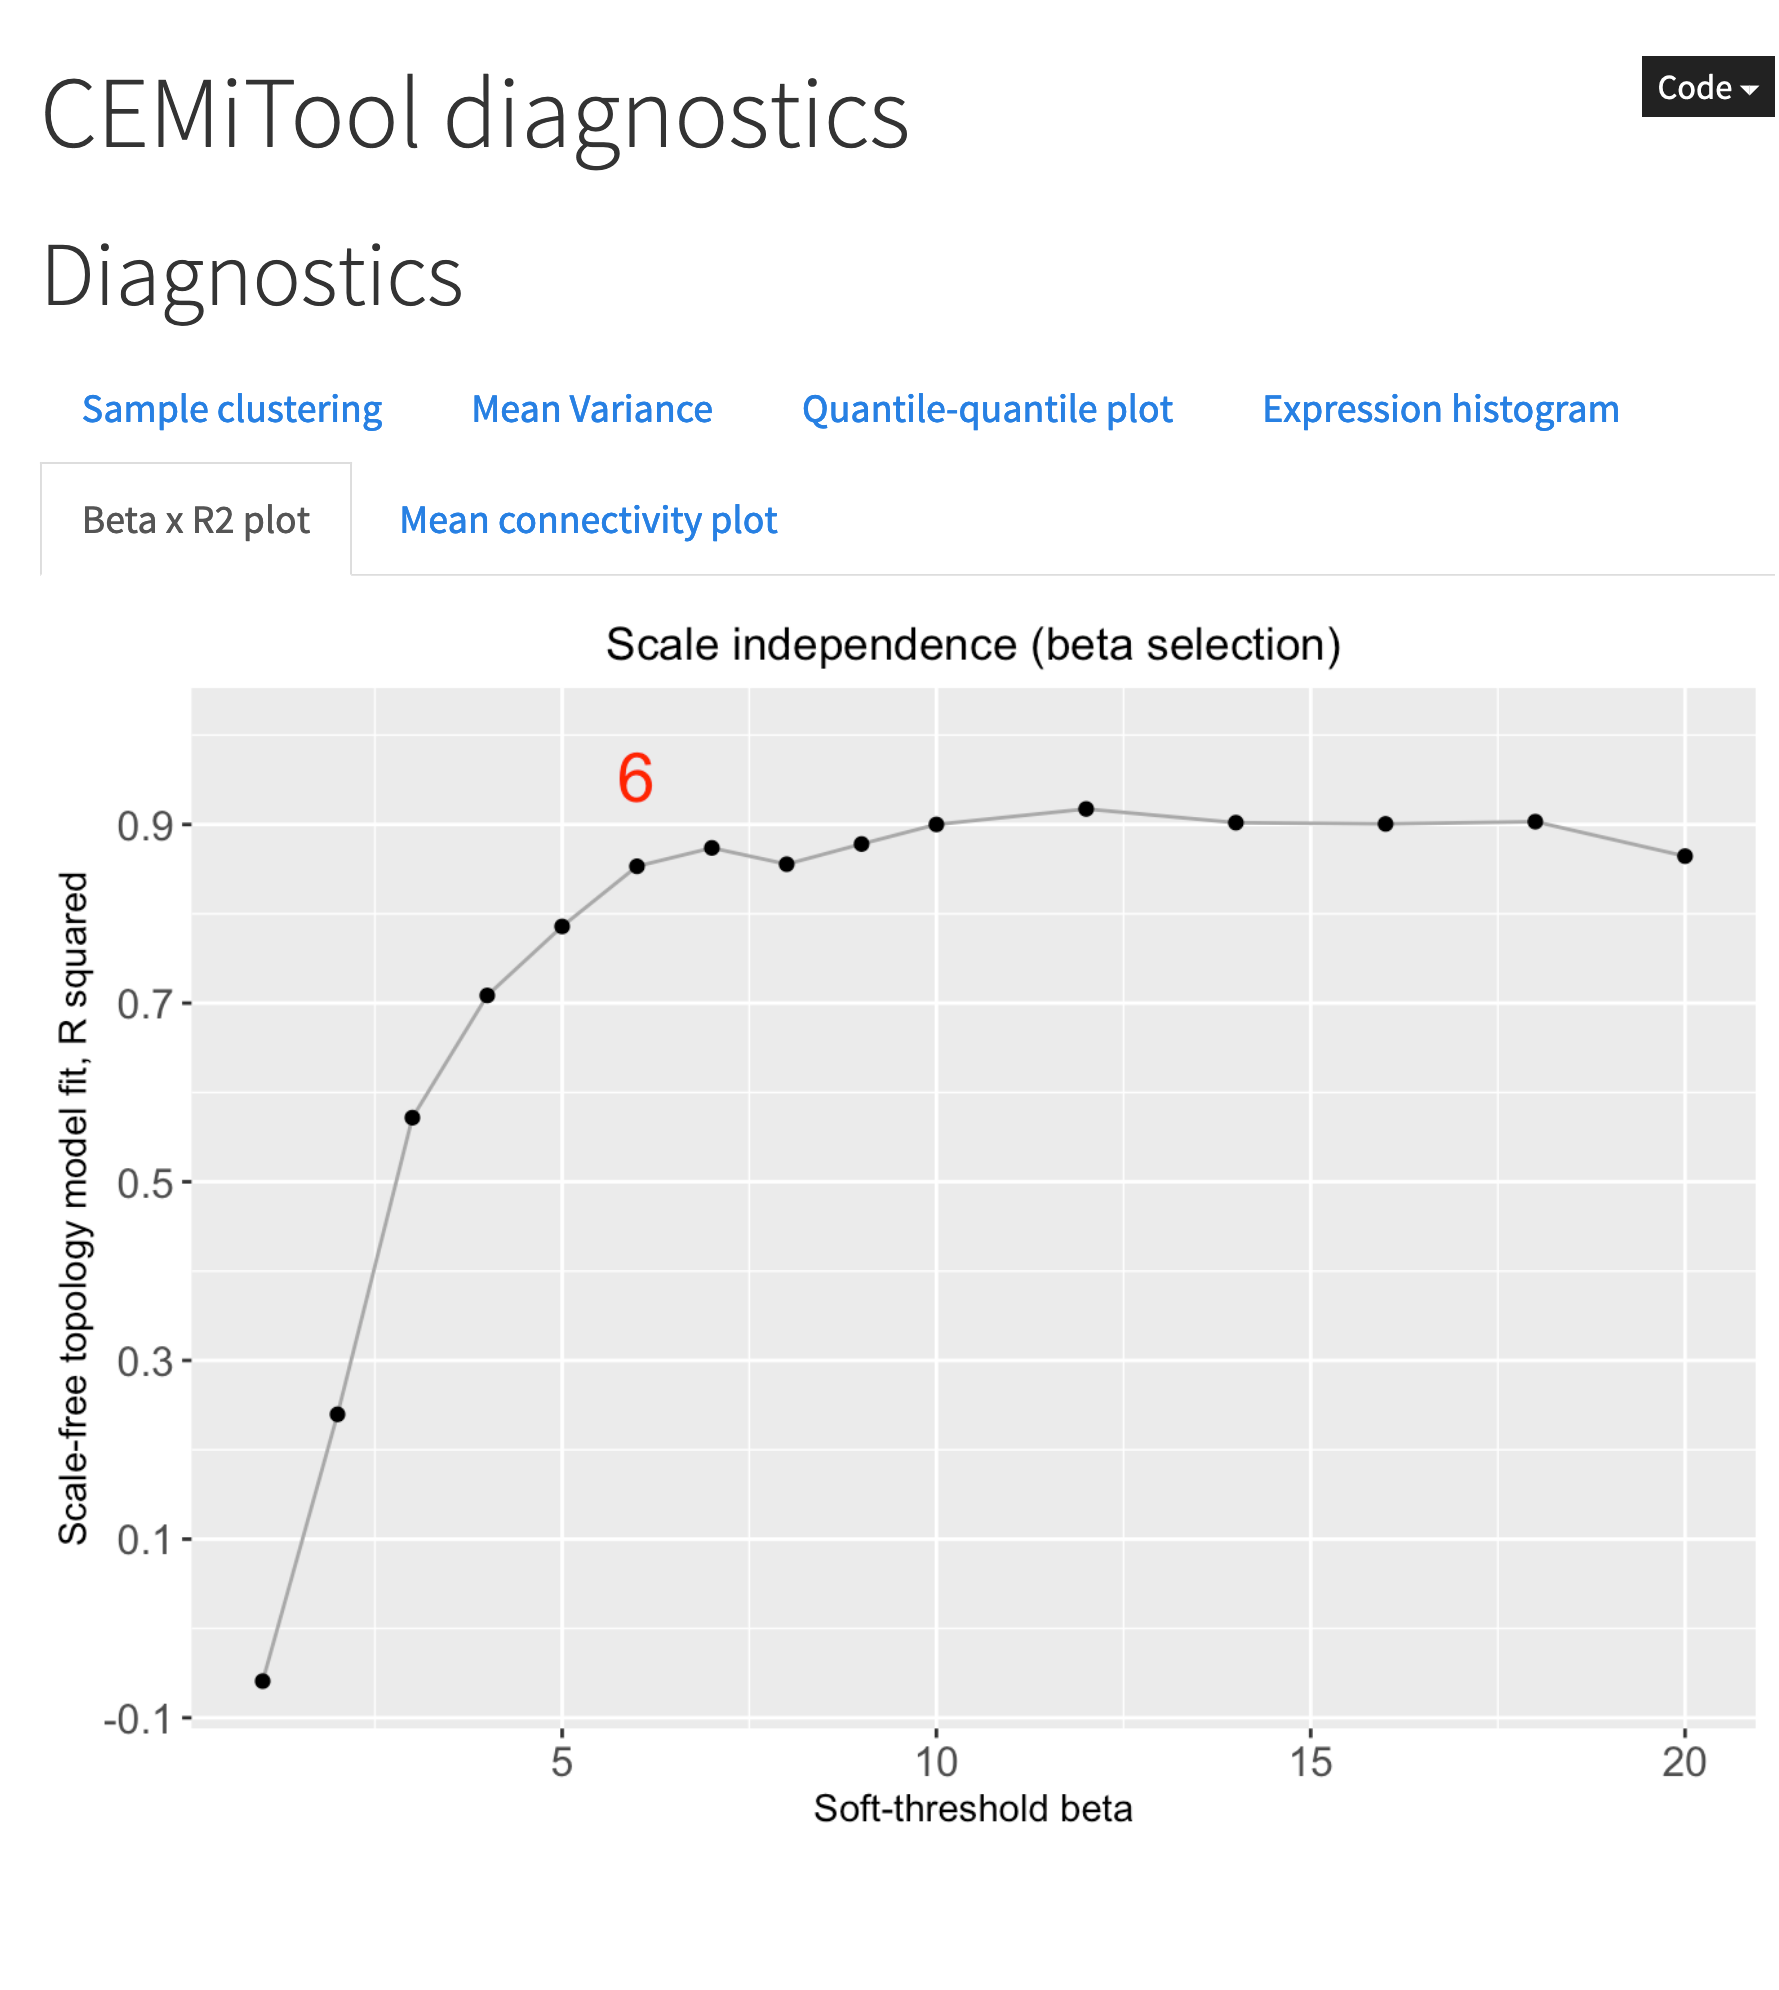
\includegraphics[width=0.9\linewidth]{images/cemi-diagnostics}
  \end{subfigure}

\caption{CEMiTool report and diagnostics HTML files.}
\label{fig:cemi-htmls}
\end{figure}


Plotting functions can always save their results to PDFs, and CEMiTool can automatically generate all plots and store them to a folder. CEMiTool can generate ten different types of plots, which include:
\begin{itemize}
  \item \texttt{plot\_sample\_tree}: Displays similarities between samples in the expression data with a dendrogram. This can be used to quickly analyze connectivity.
  \item \texttt{plot\_profile}: Compares module gene expression profiles along samples and highlights eigengenes. These plots can simplify module characterization.
  \item \texttt{plot\_beta\_r2}: Compares soft-thresholding values $\beta$ and its corresponding $R^2$ value. This plot helps in interpreting the choices of the automatically selected $\beta$ value.
  \item \texttt{plot\_mean\_k}: Graphs mean connectivity of genes in the network as a function of $\beta$. 
  \item \texttt{plot\_hist}: Plots a histogram of the distribution of gene expression. This can be used to assess data normality.
  \item \texttt{plot\_mean\_var}: Scatter plots the mean by the variance of gene expression. With RNA sequencing data this plot can be evaluated for a linear relationship.~\cite{cem-docs}
\end{itemize}

\noindent All of these plots are already displayed in the report and diagnostics files. Some plots can only be generated if additional files are included in the initial \texttt{cemitool} function call. 

One important goal of this investigation was to generate a dendrogram that displays similarities between genes, rather than samples. No function for this exists in CEMiTool and the package lacks documentation for proper creation of custom plots. As a result, there hasn't yet been successful at properly generating gene dendrograms from \texttt{cemitool} objects. This would take more time to develop and would significantly simplify output comparisons between WGCNA and CEMiTool outputs within the scope of this paper.

\subsection{Necessary Preprocessing}
\label{subsec: preprocessing}
Though CEMiTool is designed to automate most of the clustering process, it still adheres to the general concept of "garbage in, garbage out." The input dataset must have high-quality and relatively unbiased data, otherwise the output result could be very inaccurate. Ensuring data quality adds steps of necessary preprocessing, which often comes in the form of additional checks and filters -- as is the case in this report. 

With our example dataset, which contained gene data for bird samples, three filters were performed before the data was passed into the \texttt{cemitool} function:
\begin{enumerate}
  \item \emph{Sample Information:} Bird types were filtered such that only bird samples labeled with "areaX" were included in the dataset. This ensured that all samples were of the same type. Labels were stored in a separate file. With the dataset in use for this paper, this reduced the number of samples from 54 to 27.
  \item \emph{NA \& Sum Filtering:} Empty cells (cells with NA/NaN values) are replaced with zeroes, all genes were summed for each sample, and samples with sums outside a certain tolerance were dropped from the dataset. This ensures that samples overwhelmed with empty cells or irregular data are removed. With the dataset in use for this paper. this reduced the number of samples from 27 to 26.
  \item \emph{Standard Deviation Filtering:} All genes with values greater than two standard deviations outside the other data in the sample causes the entire gene to be removed. This controls for abnormal and poor data. With the dataset in use for this paper, this reduced the number of genes from about 20,000 to about 17,000. 
\end{enumerate}

Time didn't permit extensive testing of this method, but a potentially more effective and more autonomous strategy for dataset cleanup and filtering might have been through various functions available in the GWENA co-expression analysis tool.~\cite{gwena} These functions, such as \texttt{filter\_low\_var}, are intended to perform this task. When first implemented in this project, the function failed to remove any data from the dataset, however.

\subsection{R-Python Interface}
\label{subsec: interface}
The package \texttt{rpy2} was used to interface with R in Python. This package can convert seamlessly between R and Python data structures, import R packages, and fully access R objects and functions. In Python, importing CEMiTool takes only a few lines:

\begin{example}
  from rpy2.robjects.packages import importr
  
  cemitool = importr('CEMiTool')
  doParallel = importr('doParallel')

  doParallel.registerDoParallel(cores = ...)
\end{example}

\noindent From there, data can be loaded with \texttt{pandas} and fed directly into the c\texttt{cemitool} object's methods -- all of which share the same name as within the original package. This can be seen with CEMiTool's methods:

\begin{example}
  import pandas as pd

  preprocessed_dataframe = pd.read_csv(...)
  cem = cemitool.cemitool(preprocessed_dataframe, plot=True)

  cemitool.generate_report(cem) # command mirrors format in R
  cemitool.modules(cem)
  ...
\end{example}

\noindent As a result, all features and packages available in R are now put in reach of Python code with relatively minimal effort. Scripts in this project use this functionality to load and preprocess the input dataset with Python packages and operations before being run in CEMiTool, which is implemented in R. This largely neglects the flexibility brought by a Python implementation, but nevertheless displays the relatively seamless interaction between languages that \texttt{rpy2} enables. 

\subsection{Creating a Workflow}
With all of the aforementioned pieces in place, a simple workflow could be developed in Python. This workflow would take a dataset, preprocess it, run it through CEMiTool, and generate plots, reports, and diagnostics. This workflow was implemented both as a Python script and as a Jupyter Notebook. The script can be configured from within and run from the command line, and the notebook is also configured from within and can be run both locally and in Google Colab. Both implementations are available in the project repository, in the \texttt{workflow/} folder, along with a link to Google Colab. Examples of both can be seen in Figure~\ref{fig:workflow}

\begin{figure}[!htb]

  \begin{subfigure}{0.5\textwidth}
    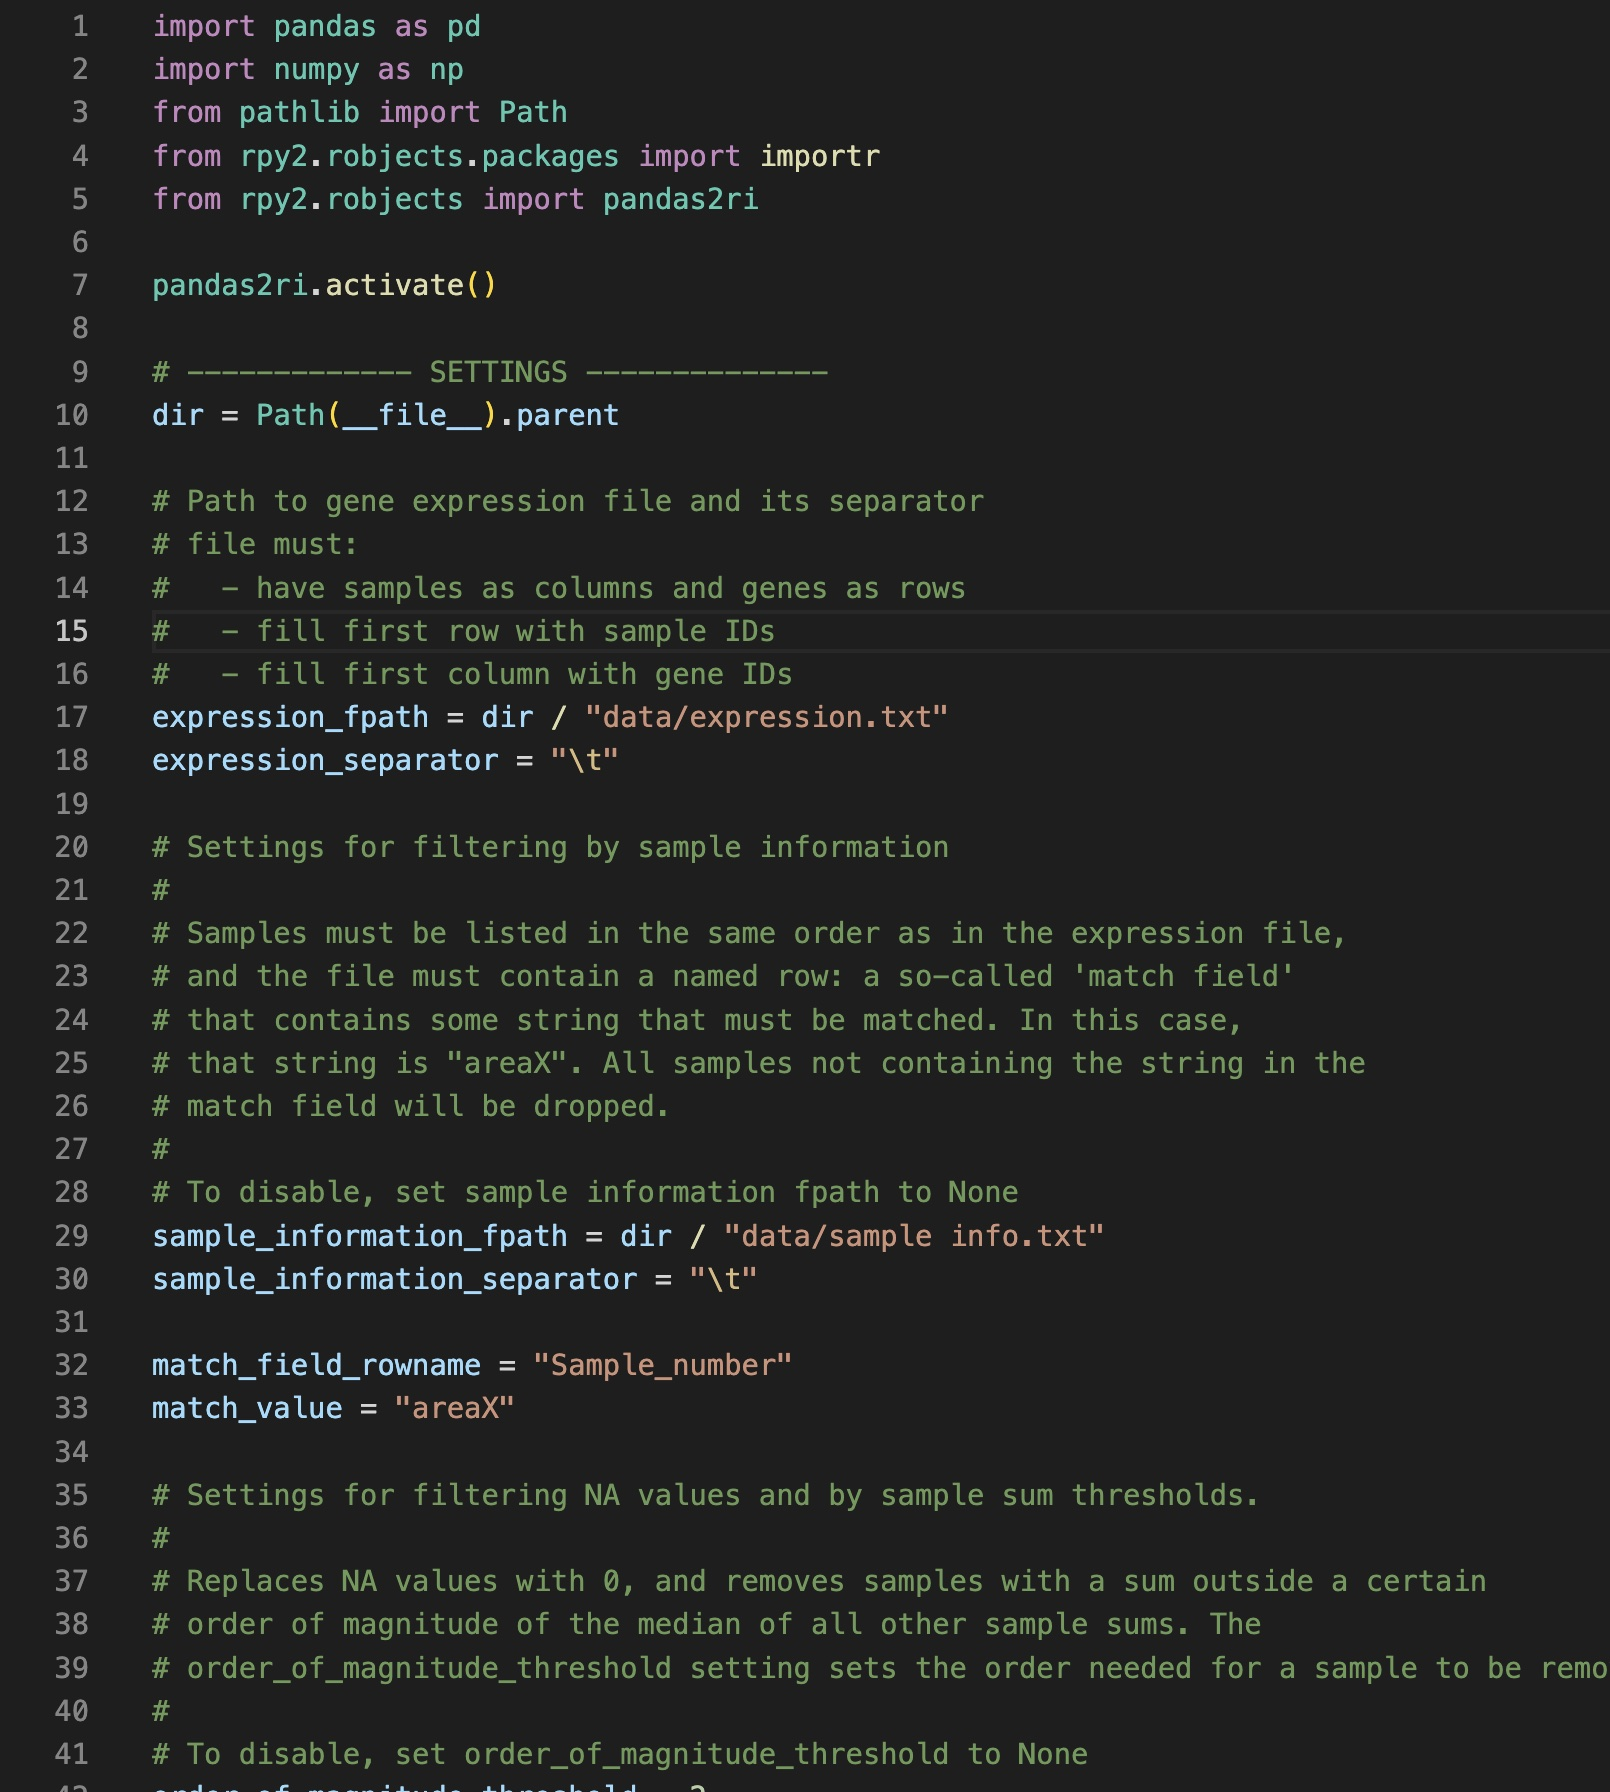
\includegraphics[width=0.95\linewidth]{images/script} 
  \end{subfigure}
  \begin{subfigure}{0.5\textwidth}
    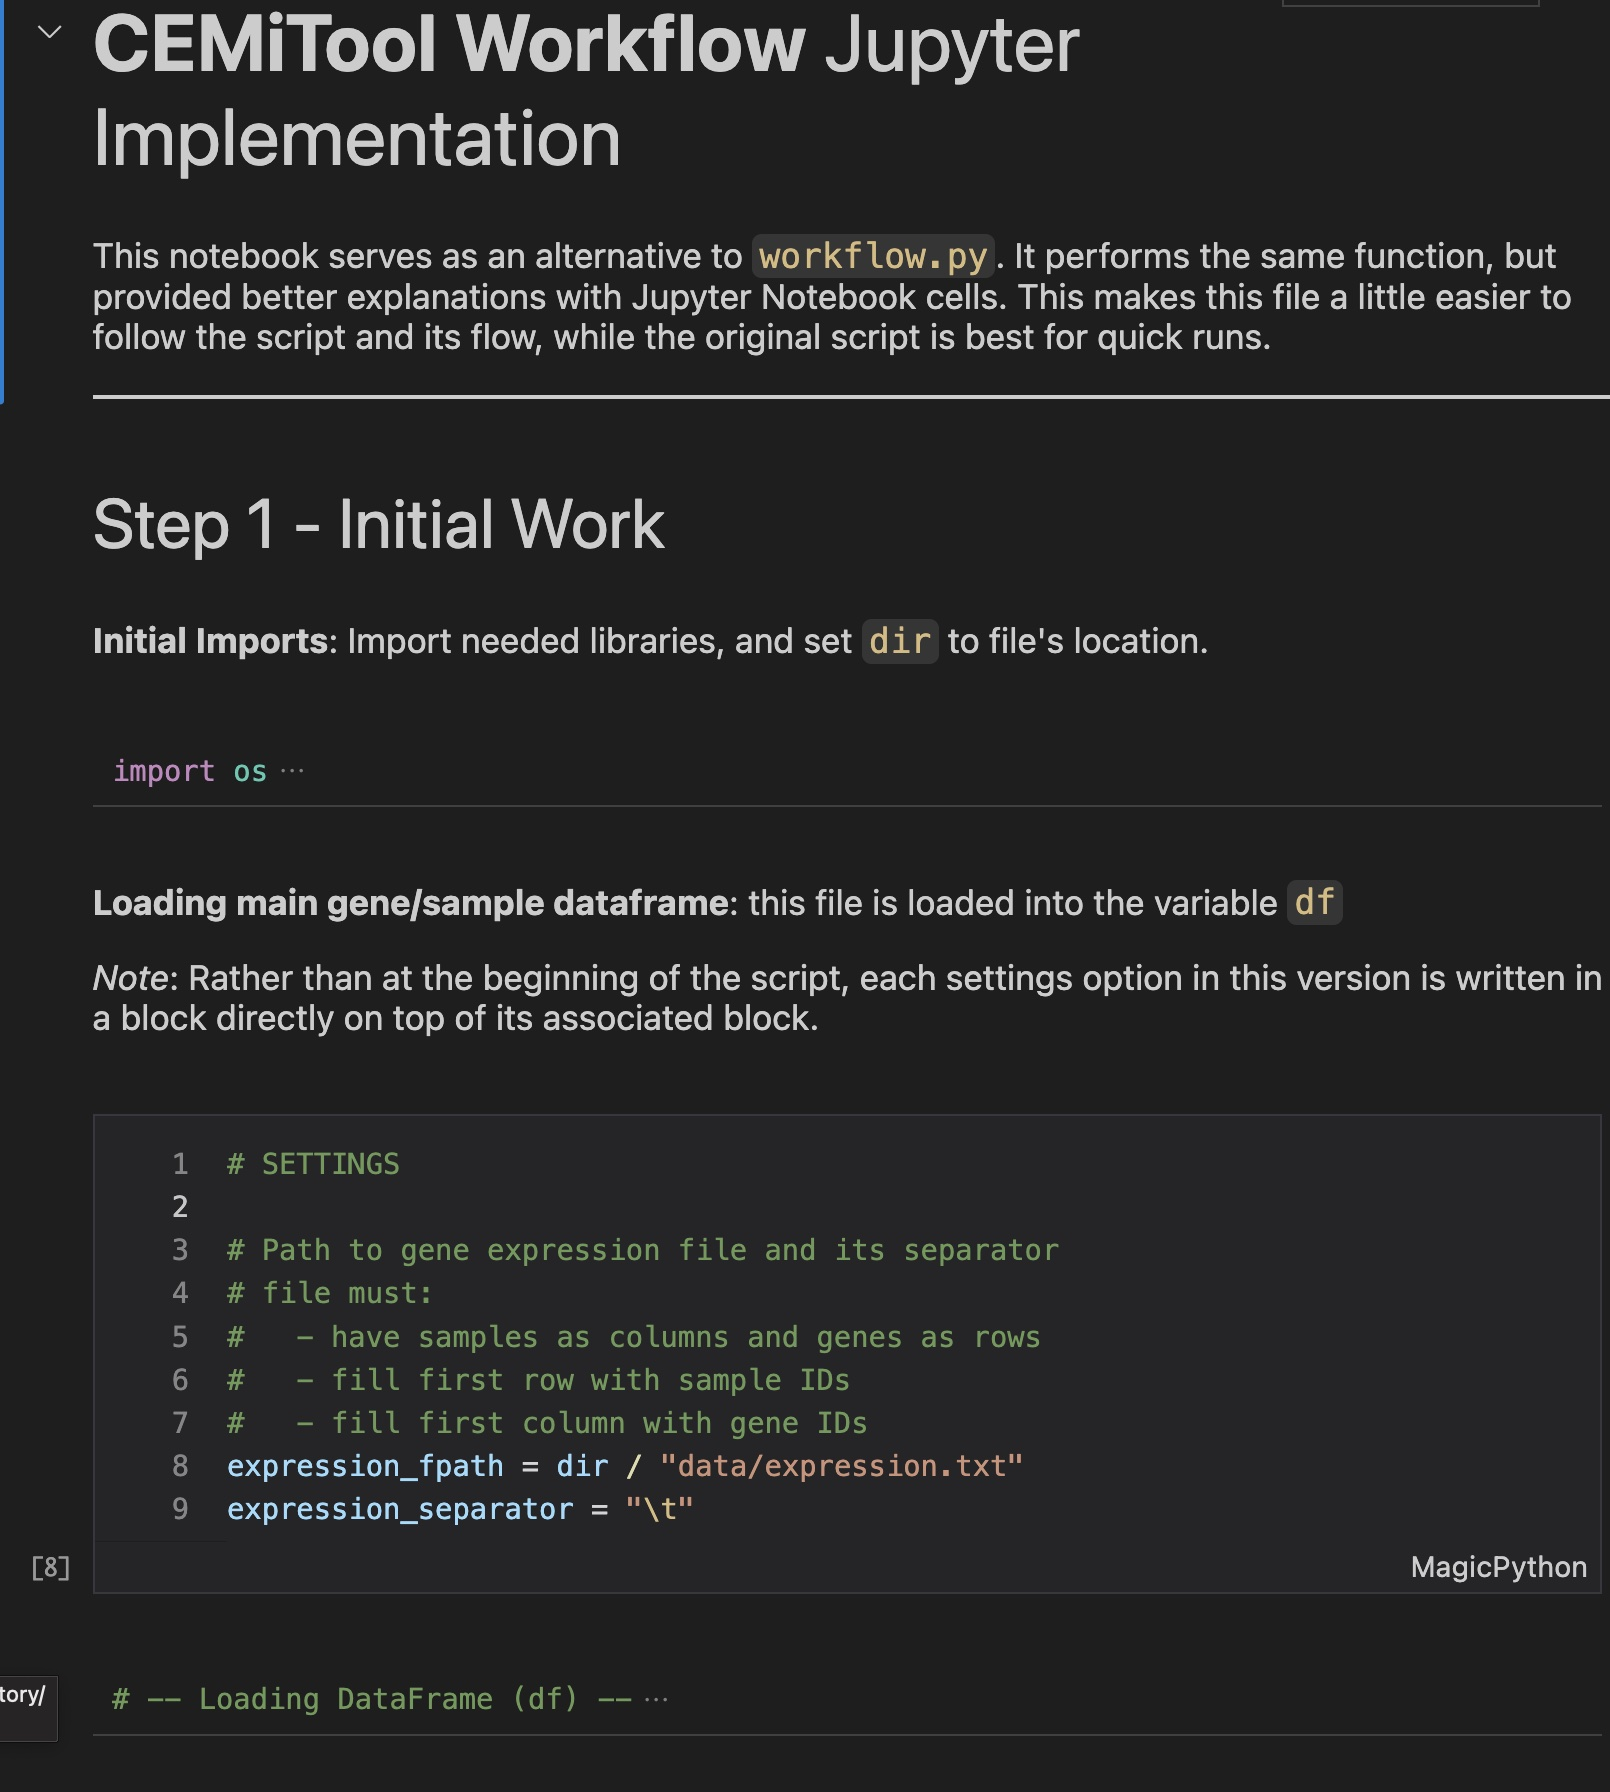
\includegraphics[width=0.95\linewidth]{images/jupyter}
  \end{subfigure}

\caption{Python script and Jupyter Notebook implementations of the workflow.}
\label{fig:workflow}
\end{figure}

\subsection{Figures \& Comparisons}
\label{subsec: comparisons}
All tests done in this investigation were done with microarray data from singing zebra finches obtained from a \emph{Neuron} paper.~\cite{dataset} The dataset and sample info used is provided in the \texttt{workflow/data/} folder. This data was run with the provided workflow, with all four types of filtering enabled (including experimental GWENA). A sample run of this dataset is provided in the \texttt{workflow/example\_output} folder. Some plots from this run are included in this report, seen in Figure~\ref{fig:beta_r2}, Figure~\ref{fig:sample_tree}, and Figure~\ref{fig:profile}.

\begin{figure}[!htb]
    \centering
    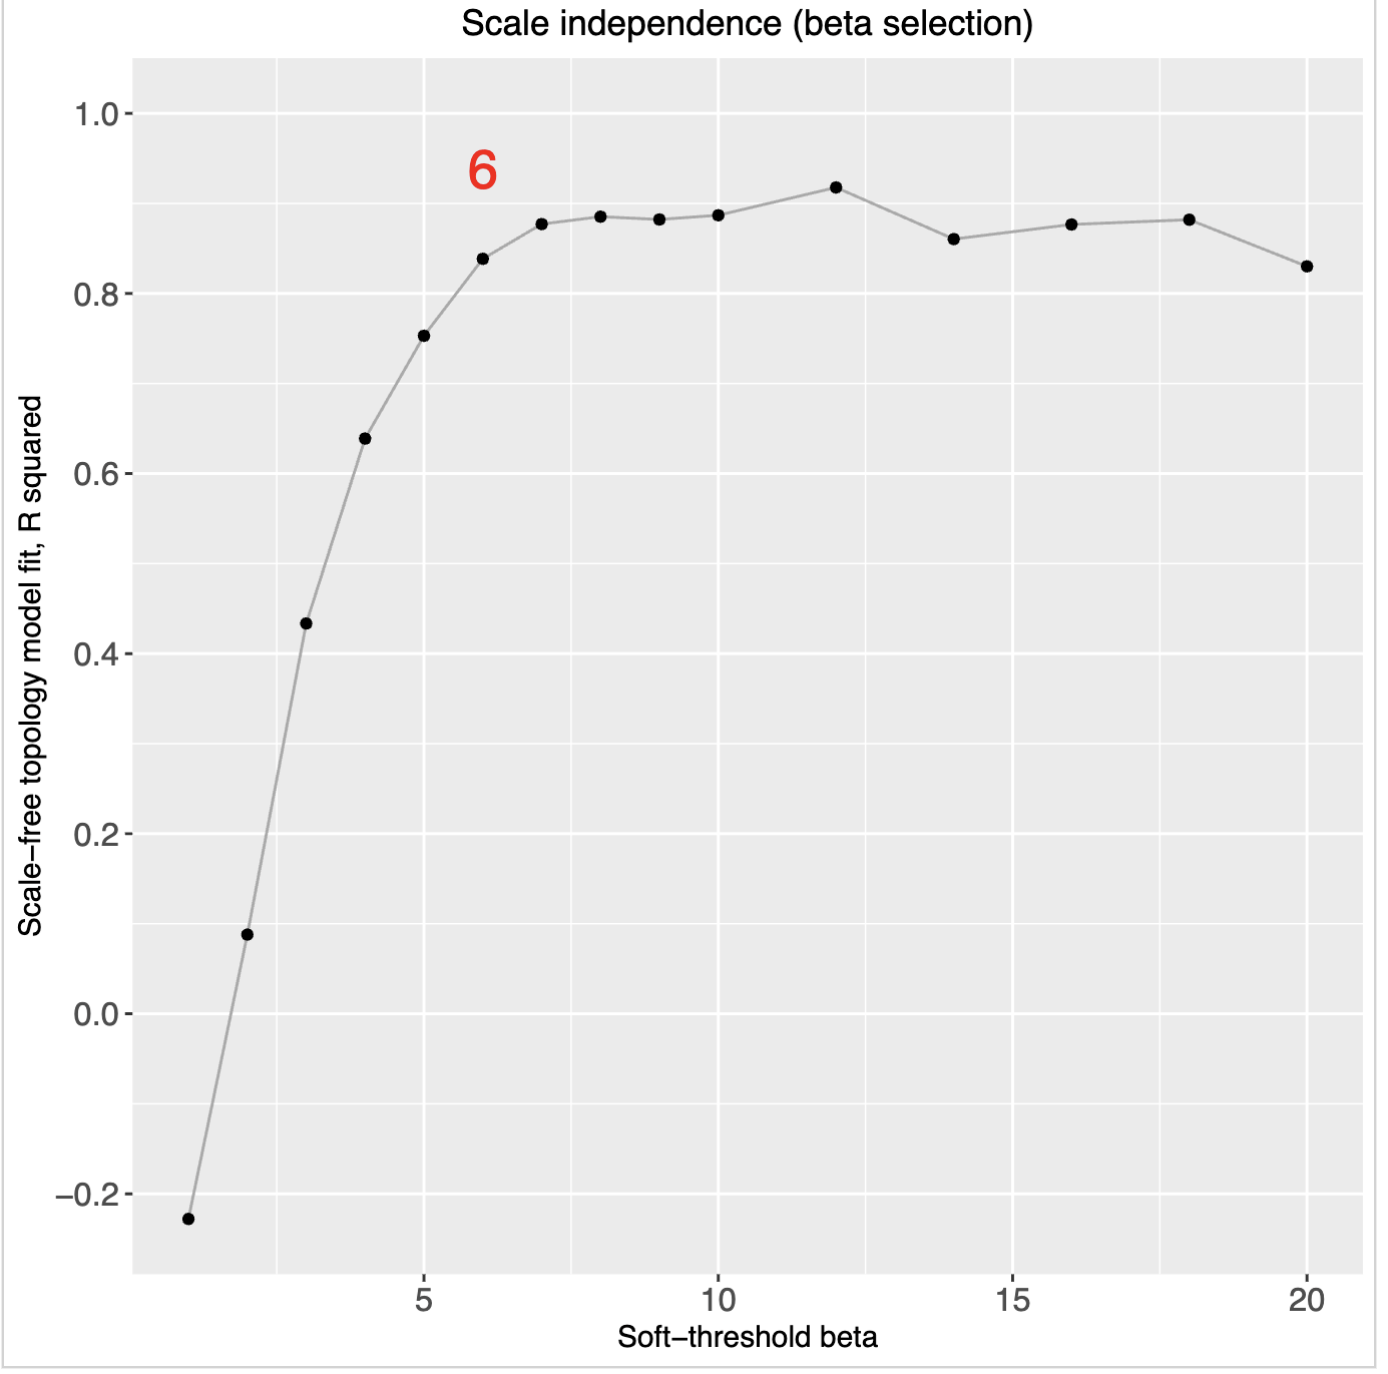
\includegraphics[width=0.7\linewidth]{images/beta_r2_plot}
    \caption{The \texttt{plot\_beta\_r2} output for the example dataset.}
    \label{fig:beta_r2}
\end{figure}

\begin{figure}[!htb]
    \centering
    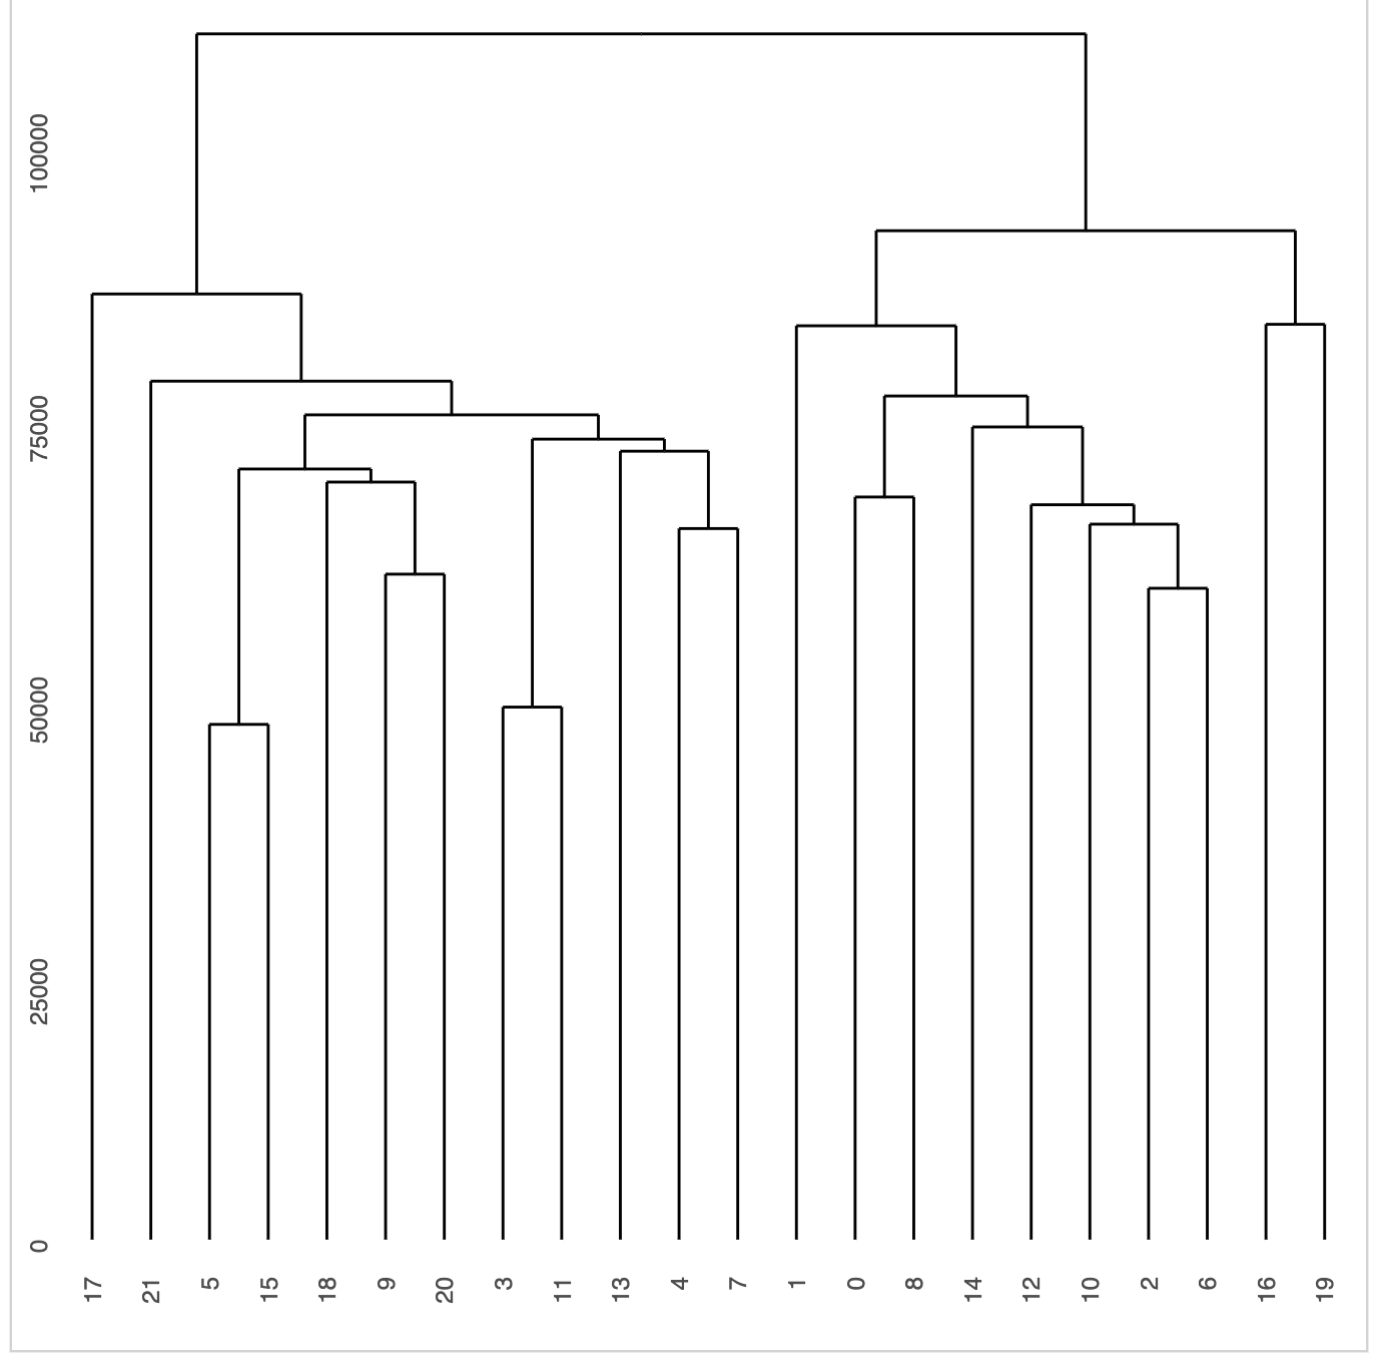
\includegraphics[width=0.7\linewidth]{images/sample_tree_plot}
    \caption{The \texttt{plot\_sample\_tree} output for the example dataset.}
    \label{fig:sample_tree}
\end{figure}

\begin{figure}[!htb]
    \centering
    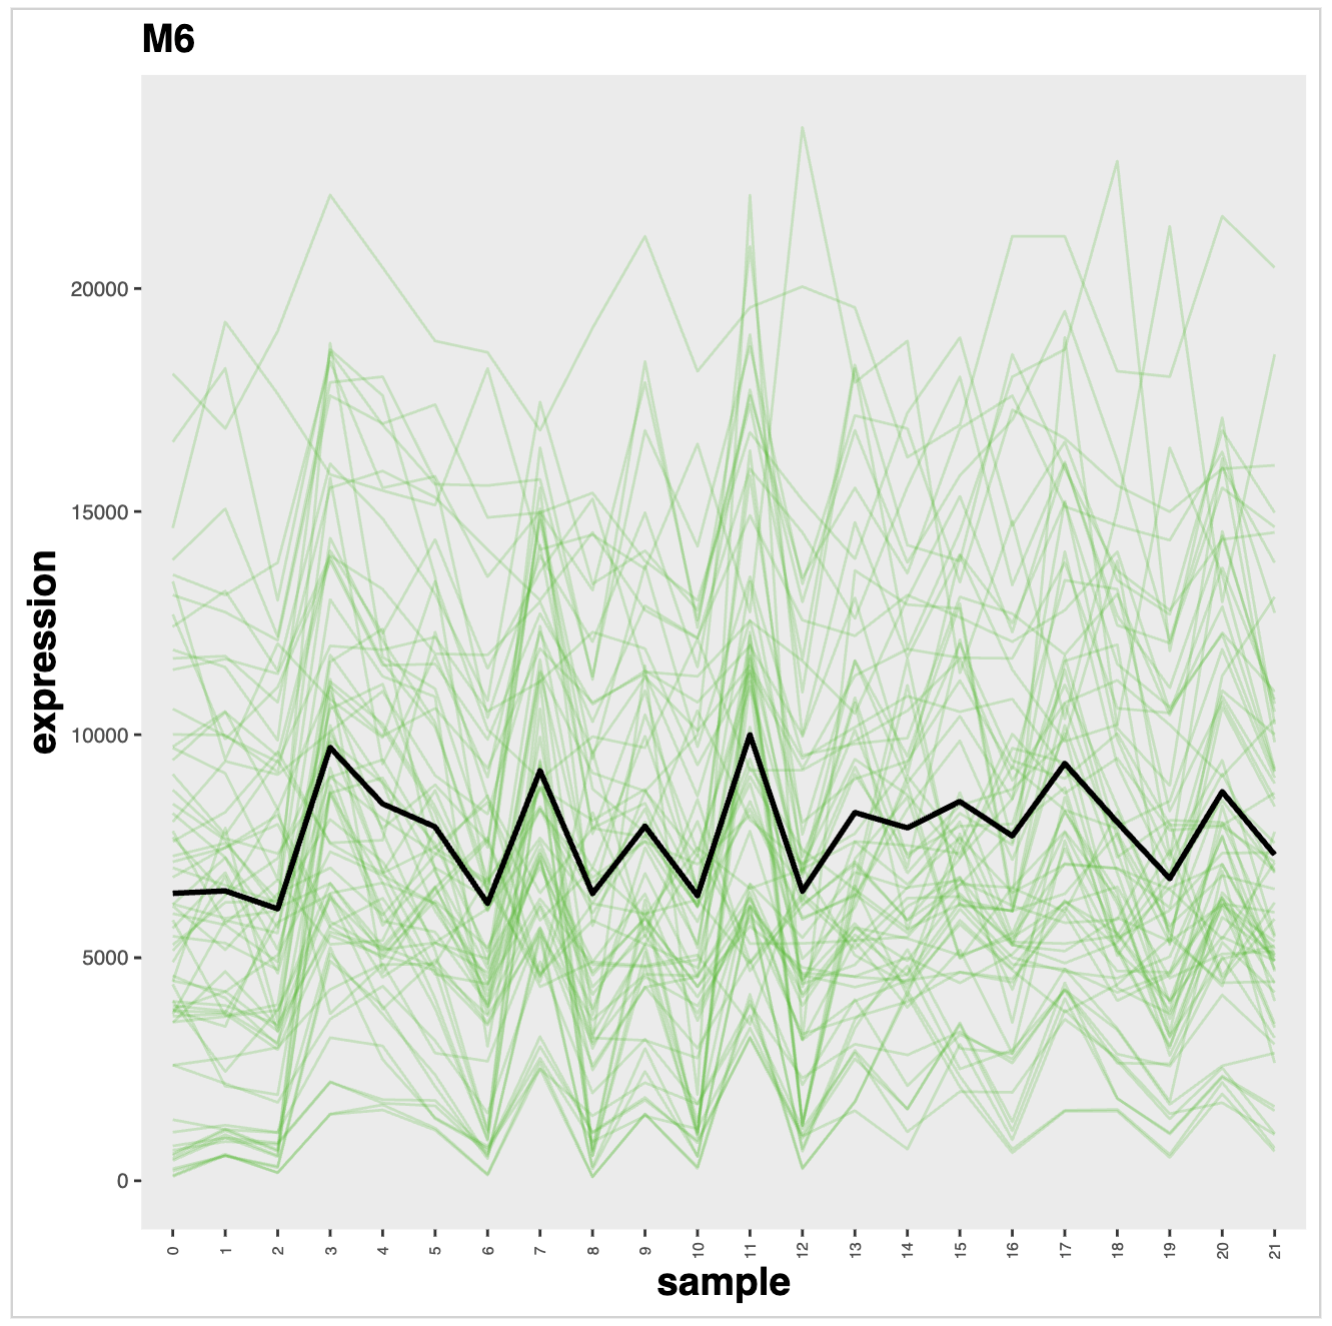
\includegraphics[width=0.7\linewidth]{images/profile_plot}
    \caption{One of the 9 \texttt{plot\_beta\_r2} outputs for the example dataset. One plot is generated for each module made, plus one more for uncorrelated genes.}
    \label{fig:profile}
\end{figure}

No plot types can yet be generated to allow for simple comparison with WGCNA data, and as a result the efficacy of the generated data cannot be compared to WGCNA. This misses the mark on a major goal of this project. To attempt to alleviate this issue, implementation work was begun on a gene dendrogram, as discussed in \ref{subsec: visualizing}. Right now, this implementation doesn't work and produces results that do not make sense. This implementation can be seen in the \texttt{extras/dendrogram-testing.ipynb} file, and an example of its plot generated from the sample data can be seen in Figure~\ref{fig:dendrogram}.

\begin{figure}[!htb]
    \centering
    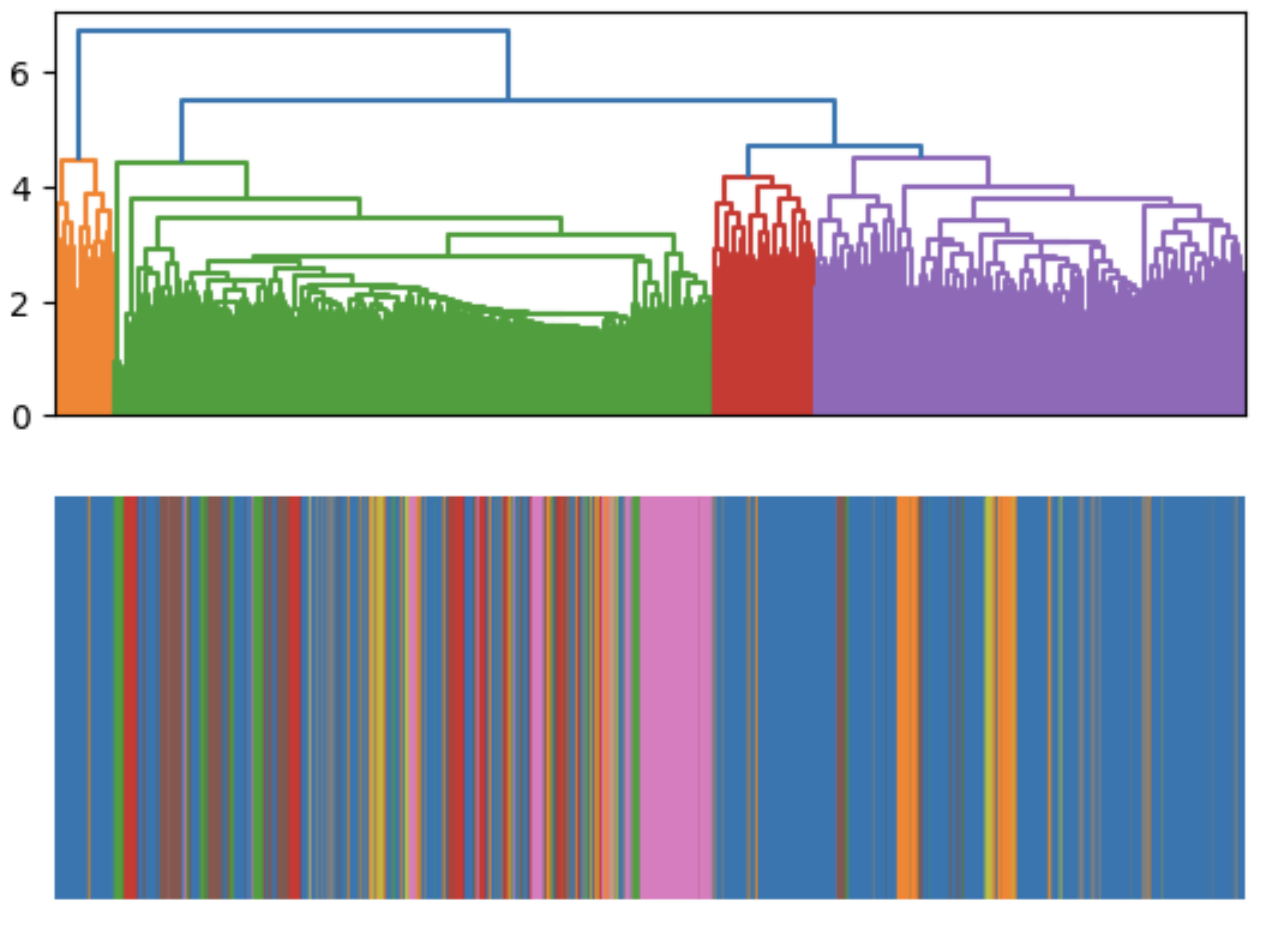
\includegraphics[width=0.7\linewidth]{images/my_dendrogram}
    \caption{The output of the custom gene dendrogram implementation with the sample dataset. The dendrograph is shown on the top, and the module associated with each leaf of the dendrogram is color-coded on the bottom.}
    \label{fig:dendrogram}
\end{figure}

\FloatBarrier

\section{Discussion}

This project made significant progress with CEMiTool, establishing a general workflow and beginning to produce results. However, with more time, there is significant room for advancement. The area that most needs work is in comparison with WGCNA results. This is completely lacking from this project, as nearly all time was spent interfacing with CEMiTool and working to obtain proper outputs. With more time, CEMiTool can be extended in ways that meet our needs for comparison, such as with gene dendrograms as seen in \ref{subsec: visualizing}, \ref{subsec: comparisons}, and in Figure~\ref{fig:dendrogram}. Other methods of comparison between CEMiTool and WGCNA were already seen in CEMiTool's original paper \cite{cem}, and with more time these methods could be explored and implemented as well. 

In addition to increased capacity for comparison, more time could be spent exploring other package options and solutions. For example, the newer package GWENA \cite{gwena} was found near the end of the investigation and, as such, could only contribute to the preprocessing methodology in \ref{subsec: preprocessing}. Other packages could ease the need for custom implementations such as the gene dendrogram, as these needs may be already implemented in these packages. 

Finally, with more time, the \texttt{rpy2} R-Python interface shown in \ref{subsec: interface} could be further taken advantage of. This could be done in a number of ways, such as those mentioned in \ref{subsec: python-intro}. The benefits of implementing this workflow in Python will become most apparent as the project is scaled up and begins to require increased generality, more robust package support, and a wider array of external modules.

Nevertheless, the advantages of more modern packages like CEMiTool are clear: this workflow is very short and readible. With WGCNA, the same task would take much more code, parameterization, and overall effort. If it is made clear that CEMiTool's results (or some other package) are comparable in quality to WGCNA, this simplified workflow will substantially increase the ease of future clustering work in research both inside and outside neuroscience applications.


\bibliography{koppe}

\address{Benjamin Koppe\\
  University of Arizona\\
  Department of Computer Science\\
  United States\\}
\email{koppe@arizona.edu}

\address{Dr. Charles Higgins\\
  University of Arizona\\
  Department of Neuroscience\\
  Department of Electrical Engineering\\
  United States\\}
\email{cmh@arizona.edu}